\documentclass[a4paper]{article}
\usepackage{lipsum} %This package just generates Lorem Ipsum filler text. 
\usepackage{fullpage} % changes the margin
\usepackage{mathpazo}
\usepackage{multicol}
\usepackage{enumerate, eucal}
\usepackage{amsmath,amsfonts,amsthm, amssymb} % Math packages

\usepackage{listings}
\usepackage{xcolor}
\usepackage{graphicx}
\usepackage{attachfile}
\usepackage{geometry}
\geometry{a4paper, scale=0.9}

\begin{document}
%Header-Make sure you update this information!!!!
\noindent
\large \textbf{Homework 1} \hfill \textbf{Xun Gong(517020910141} \\
\normalsize {\bf CS 259 @ SJTU} \hfill ACM Class, Zhiyuan College, SJTU\\
Prof.~{\bf David Bindel} \hfill Due Date: May 29, 2019\\
TA.~{\bf Zhou Fan} \hfill Submit Date: \today

\section*{Problem 1: Stochastic gradient descent}

\subsection*{(1)}

Code is in attachment. \attachfile{code.py}
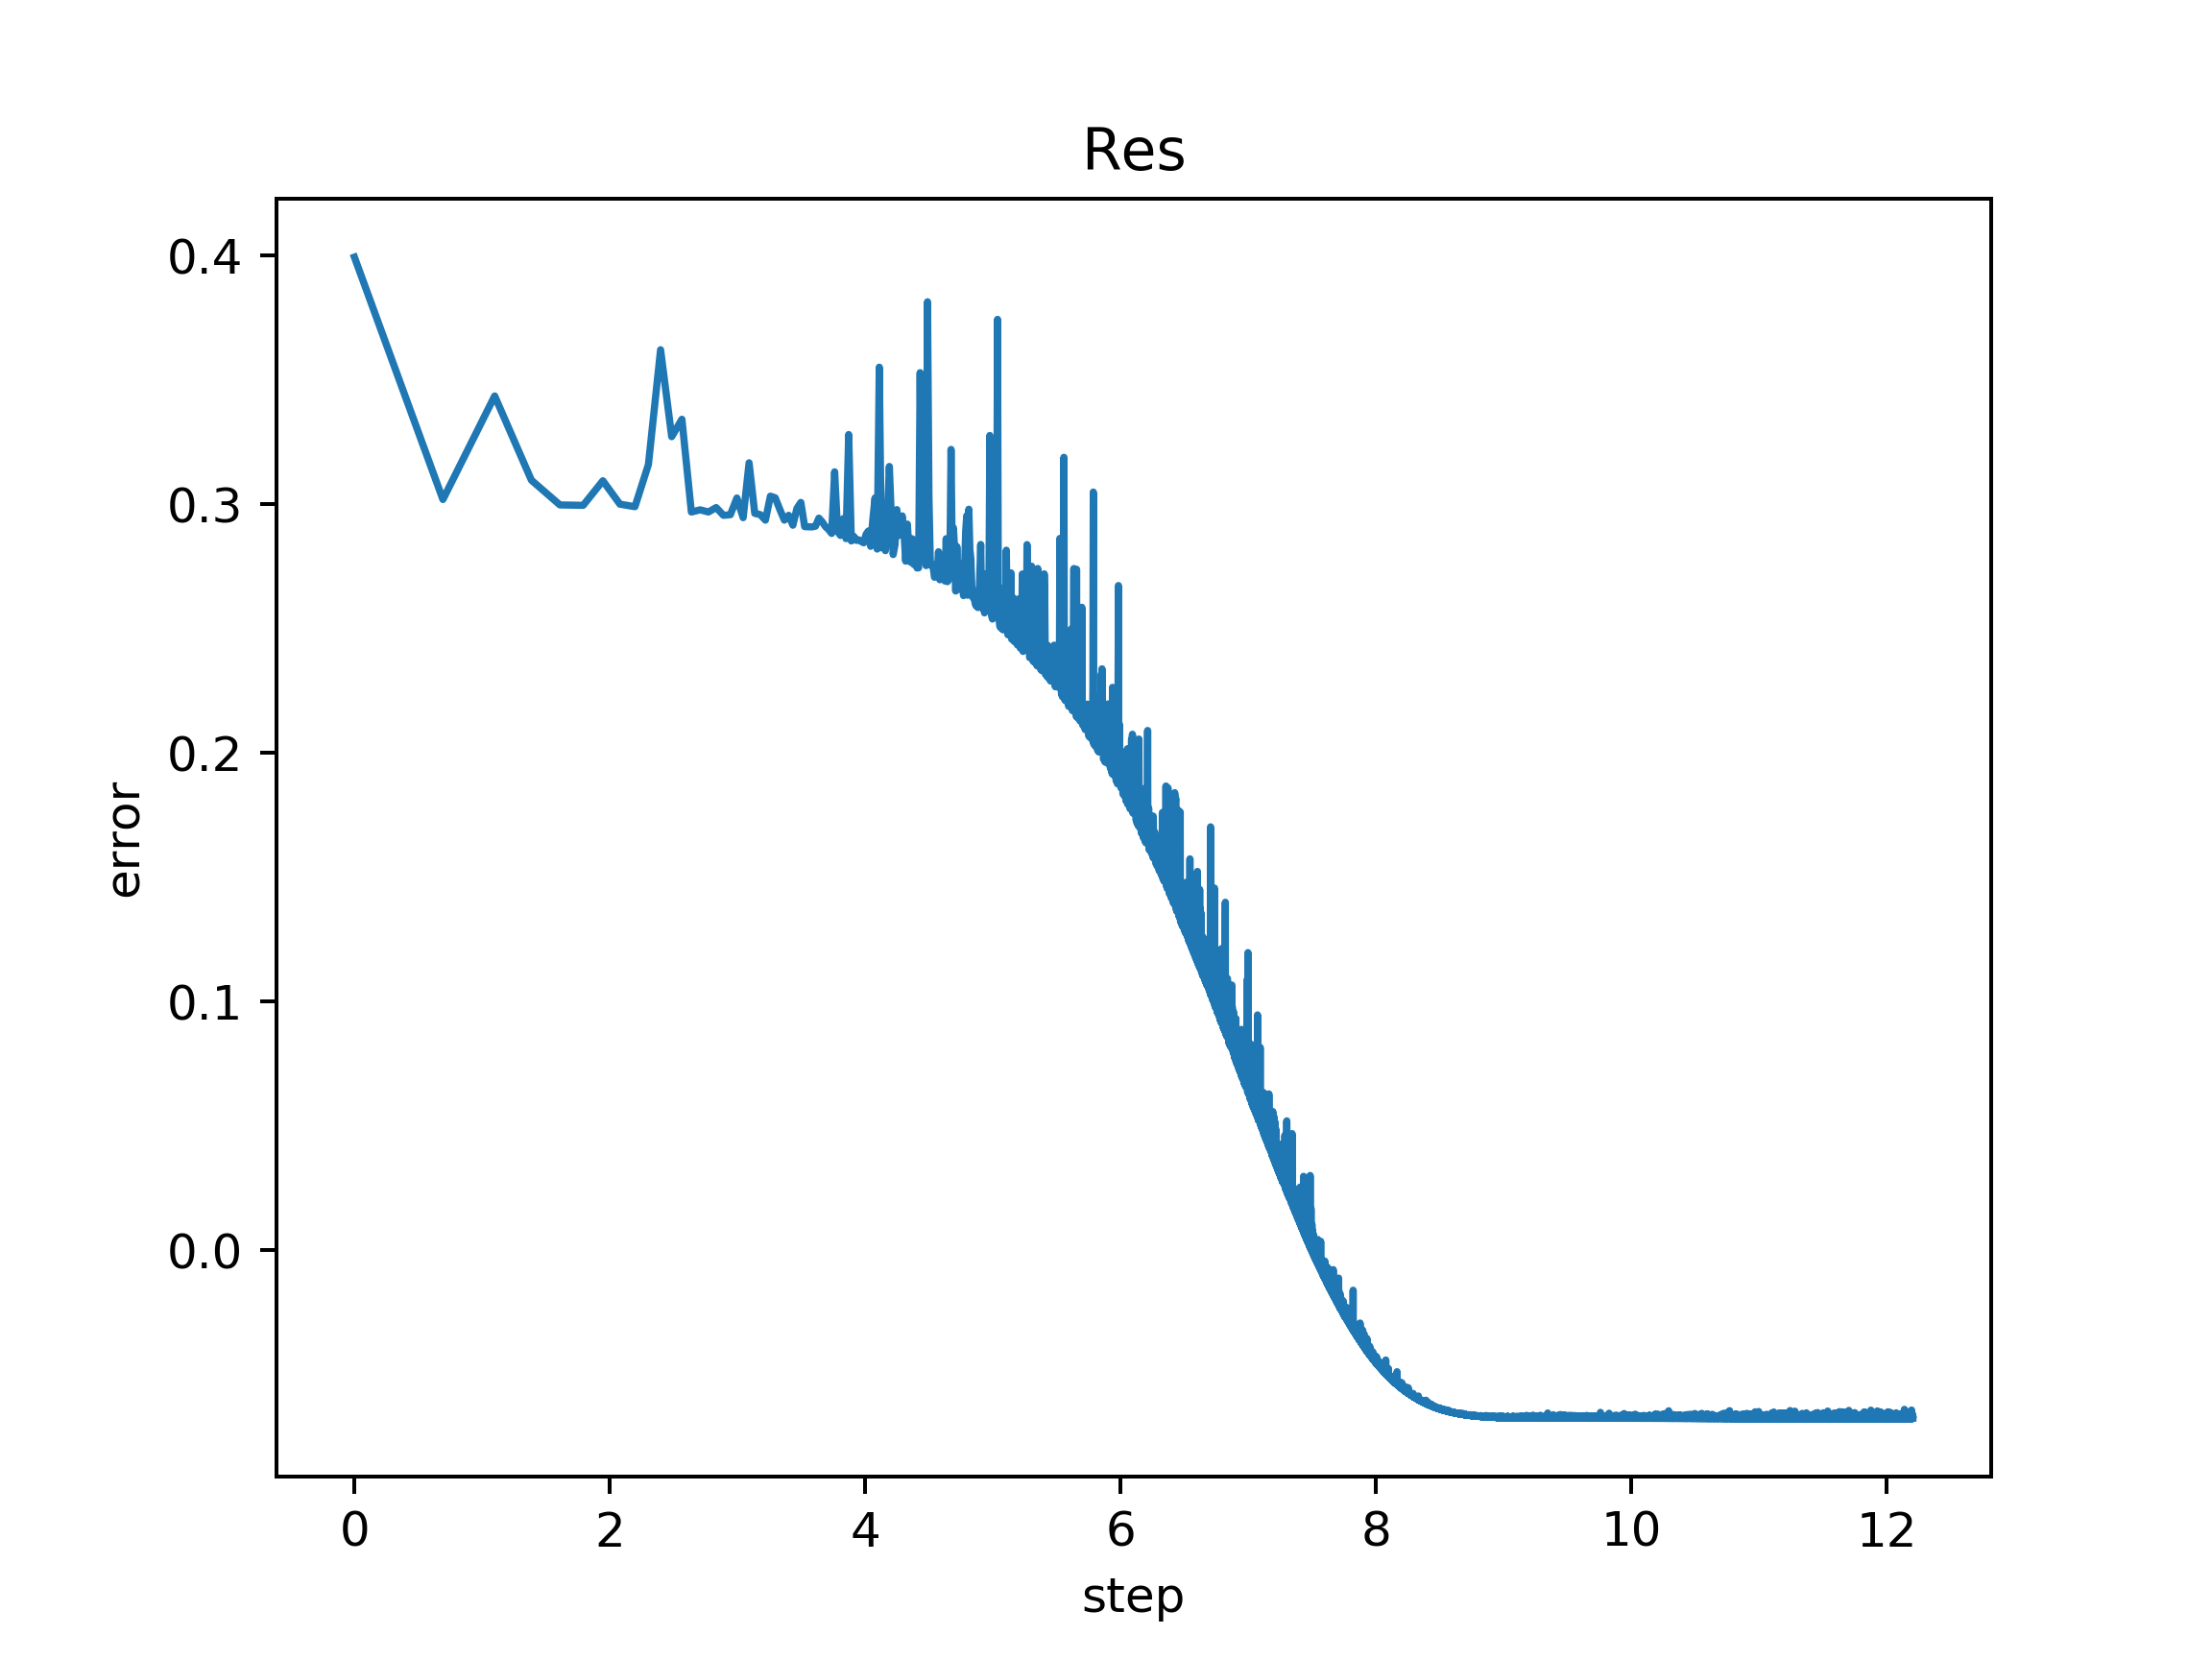
\includegraphics[scale=0.6]{hw.png}

\subsection*{(2)}

Rule: Stochastic gradient descent is converge to $0$.


\section*{Problem 2: Least 2p-norm regression}

\subsection*{(1)}

$$f(x) = \begin{pmatrix}
    \frac{1}{\sqrt{p}} r_1^p \\
    \cdots \\
    \frac{1}{\sqrt{p}} r_n^p \\
\end{pmatrix},\quad r_i = (b - Ax)_i = b_i - A_{i,:}x $$

$$J(x) = - \sqrt{p} \begin{pmatrix}
    r_1^{p-1} a_{1, 1} &\cdots& r_1^{p-1} a_{1, n} \\
    &\cdots& \\
    r_n^{p-1} a_{n, 1}& \cdots & r_b^{p-1} a_{n, n}\\
\end{pmatrix}$$

\subsection*{(2)}

Equal to show Gauss-Newton Step $\equiv min||D^k(Ap^k-r^k)||^2$
\begin{align*}
    & \mathcal{L} = ||D^k(Ap^k - b + Ax||^2 \\
    & \delta \mathcal{L} = \delta (D^k(Ap^k - b + Ax)^T(D^k(Ap^k - b + Ax) \\
    & \delta \mathcal{L} = 2 \delta x^T D^2 (A^TAx - A^Tb + A^T A p) \\
    & \because \delta \mathcal{L} = 0\\
    & \therefore 0 = A^TAx - A^T b + A^T A p \\
    & p = - (A^TA)^{-1} (A^TAx - A^T b) \\
    & \text{What is interesting, } p = -[f'^Tf']^{-1} \delta \phi \\
    & \therefore \text{These 2 question has same solution.} \\
\end{align*}

$\square$


\end{document}
